\let\negmedspace\undefined
\let\negthickspace\undefined
\documentclass[journal]{IEEEtran}
\usepackage[a5paper, margin=10mm, onecolumn]{geometry}
%\usepackage{lmodern} % Ensure lmodern is loaded for pdflatex
\usepackage{tfrupee} % Include tfrupee package

\setlength{\headheight}{1cm} % Set the height of the header box
\setlength{\headsep}{0mm}     % Set the distance between the header box and the top of the text

\usepackage{gvv-book}
\usepackage{gvv}
\usepackage{cite}
\usepackage{amsmath,amssymb,amsfonts,amsthm}
\usepackage{algorithmic}
\usepackage{graphicx}
\usepackage{textcomp}
\usepackage{xcolor}
\usepackage{txfonts}
\usepackage{listings}
\usepackage{enumitem}
\usepackage{mathtools}
\usepackage{gensymb}
\usepackage{comment}
\usepackage[breaklinks=true]{hyperref}
\usepackage{tkz-euclide} 
\usepackage{listings}
% \usepackage{gvv}                                        
\def\inputGnumericTable{}                                 
\usepackage[latin1]{inputenc}                                
\usepackage{color}                                            
\usepackage{array}                                            
\usepackage{longtable}                                       
\usepackage{calc}                                             
\usepackage{multirow}                                         
\usepackage{hhline}                                           
\usepackage{ifthen}                                           
\usepackage{lscape}
\begin{document}

\bibliographystyle{IEEEtran}
\vspace{3cm}

\title{NCERT-10.3.4.2.1}
\author{EE24BTECH11055 - Sai Akhila}
% \maketitle
% \newpage
% \bigskip
{\let\newpage\relax\maketitle}

\renewcommand{\thefigure}{\theenumi}
\renewcommand{\thetable}{\theenumi}
\setlength{\intextsep}{10pt} % Space between text and floats


\numberwithin{equation}{enumi}
\numberwithin{figure}{enumi}
\renewcommand{\thetable}{\theenumi}

% Question
\section*{Question:}
If we add $1$ to the numerator and subtract $1$ from the denominator, a fraction reduces to $1$. It becomes $\frac{1}{2}$ if we only add 1 to the denominator. What is the fraction?
%  Solution
\section*{Theoretical Solution:}
Let the fraction be $\frac{x}{y}$.\\
Given, $\frac{x+1}{y-1} = 1$ and, $\frac{x}{y+1}=\frac{1}{2}$\\\\
Solving them:\\
$x+1=y-1 \implies x-y+2=0$
\begin{align}
    x-y+2=0
\end{align}
\begin{align}
  2x-y-1=0
\end{align}\\
$$y=x+2$$
$$2x - (x+2)-1=0$$
$$x=3$$
Substituting $x=3$ in equation $(0.1)$, we get $y=5$.\\
Therefore the fraction is $\frac{3}{5}$
\section*{Using LU decomposition}
LU Decomposition is used primarily to simplify the process of solving systems of linear equations and other matrix-related computations. The main reason for using LU decomposition is to break down a complex matrix operation into simpler steps. \\
The system of equations $(0.1)$ and $(0.2)$ can be written as:
\begin{align}
    A \cdot \vec{x} =\vec{b}
\end{align}
where,\\
\[
A = 
\begin{bmatrix}
1 & -1 \\
2 & -1 \\
\end{bmatrix}
\]
\[
\vec{x} =
\begin{bmatrix}
    x\\
    y\\
\end{bmatrix}
\] and
\[
\vec{b}=
\begin{bmatrix}
-2\\
1\\
\end{bmatrix}
\]
We decompose the matrix $A$ into two simple triangular matrices L (lower triangular) and U (upper triangular).\\
Instead of solving the system directly, solve two systems:\\
$L\cdot y = b$ (forward substitution)\\
$U\cdot x = y$ (backward substitution)\\
Given below are the steps for implementation of this algorithm.
\subsection*{1. Initialize $ L$ as an identity matrix and $ U $ as $ A $}

\[
L =
\begin{bmatrix}
1 & 0 \\
0 & 1
\end{bmatrix}
\]

\[
U =
\begin{bmatrix}
1 & -1 \\
2 & -1
\end{bmatrix}
\]

\subsection*{2. Perform Gaussian elimination to make $ U $ upper triangular}
For each column $j \geq k$, the entries of $U$ in the $k$th row are updated as:
\begin{align}
    U_{k,j} = A_{k,j} - \sum_{m=1}^{k-1} L_{k,m}.U_{m,j},   \forall{j \geq k}
\end{align}
For each row $i > k$, the entries of $L$ in the $k$th column are updated as:
\begin{align}
    L_{j,k} = \frac{1}{U_{k,k}}\brak{A_{j,k} - \sum_{m=1}^{k-1}.U_{m,k}}, \forall{i>k}
\end{align}

Eliminate $ U_{21} $ (second row, first column)
- The multiplier is:

\[
l_{21} = \frac{2}{1} = 2
\]

- Subtract $2$ times the first row from the second row:

\[
R_2 \rightarrow R_2 - 2R_1
\]

\[
U =
\begin{bmatrix}
1 & -1 \\
0 & 1
\end{bmatrix}
\]

- Store the multiplier in  $L$ :

\[
L =
\begin{bmatrix}
1 & 0 \\
2 & 1
\end{bmatrix}
\]

\subsection*{3. Final Result}
We have decomposed $ A $ into:

\[
L =
\begin{bmatrix}
1 & 0 \\
2 & 1
\end{bmatrix}
\]

\[
U =
\begin{bmatrix}
1 & -1 \\
0 & 1
\end{bmatrix}
\]

Thus, we have \( A = LU \).

Since \( A = LU \), we rewrite it as:

\[
LUx = b
\]

Define \( y \) such that:

\[
Ly = b
\]

This gives two triangular systems:\\
1. Solve \( Ly = b \) (Forward Substitution)\\
2. Solve \( Ux = y \) (Backward Substitution)

\section*{Step 1: Solve $ Ly = b $ (Forward Substitution)}

Expanding:

\[
\begin{bmatrix}
1 & 0 \\
2 & 1
\end{bmatrix}
\begin{bmatrix}
y_1 \\
y_2
\end{bmatrix}
=
\begin{bmatrix}
-2 \\
1
\end{bmatrix}
\]

This gives the equations:

\[
y_1 = -2
\]

\[
2y_1 + y_2 = 1
\]

Solving for $ y_2 $:

\[
y_2 = 1 - 2(-2) = 1 + 4 = 5
\]

Thus, 

\[
y =
\begin{bmatrix}
-2 \\
5
\end{bmatrix}
\]

\section*{Step 2: Solve $ Ux = y $ (Backward Substitution)}

Expanding:

\[
\begin{bmatrix}
1 & -1 \\
0 & 1
\end{bmatrix}
\begin{bmatrix}
x_1 \\
x_2
\end{bmatrix}
=
\begin{bmatrix}
-2 \\
5
\end{bmatrix}
\]

This gives the equations:

\[
x_1 - x_2 = -2
\]

\[
x_2 = 5
\]

Solving for $ x_1 $:

\[
x_1 = -2 + x_2 = -2 + 5 = 3
\]

Thus, the solution is:

\[
x =
\begin{bmatrix}
3 \\
5
\end{bmatrix}
\]

\begin{figure}[h]
    \centering
    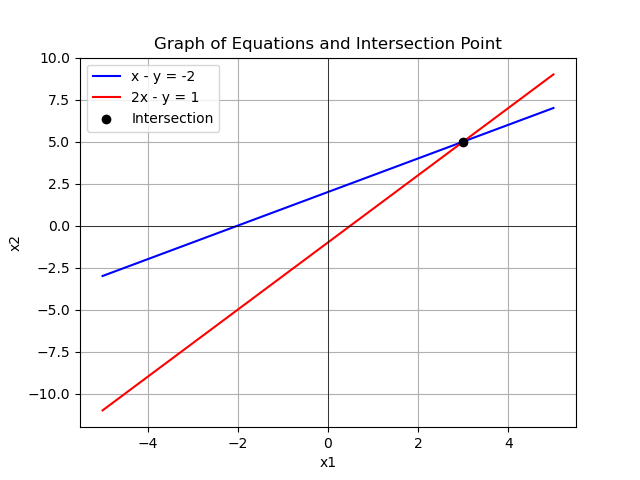
\includegraphics[width=0.8\columnwidth]{figs/lu.png}
    \caption{Graph of the equations with the intersection point}
    \label{fig:intersection}
\end{figure}

\end{document}

